\documentclass[noauthor,nooutcomes,handout,12pt]{ximera}
%\usepackage{subcaption}

\graphicspath{  
{./}
{./whoAreYou/}
{./drawingWithTheTurtle/}
{./bisectionMethod/}
{./circles/}
{./anglesAndRightTriangles/}
{./lawOfSines/}
{./lawOfCosines/}
{./plotter/}
{./staircases/}
{./pitch/}
{./qualityControl/}
{./symmetry/}
{./nGonBlock/}
}


%% page layout
\usepackage[cm,headings]{fullpage}
\raggedright
\setlength\headheight{13.6pt}


%% fonts
\usepackage{euler}

\usepackage{FiraMono}
\renewcommand\familydefault{\ttdefault} 
\usepackage[defaultmathsizes]{mathastext}
\usepackage[htt]{hyphenat}

\usepackage[T1]{fontenc}
\usepackage[scaled=1]{FiraSans}

%\usepackage{wedn}
\usepackage{pbsi} %% Answer font


\usepackage{cancel} %% strike through in pitch/pitch.tex


%% \usepackage{ulem} %% 
%% \renewcommand{\ULthickness}{2pt}% changes underline thickness

\tikzset{>=stealth}

\usepackage{adjustbox}

\setcounter{titlenumber}{-1}

%% journal style
\makeatletter
\newcommand\journalstyle{%
  \def\activitystyle{activity-chapter}
  \def\maketitle{%
    \addtocounter{titlenumber}{1}%
                {\flushleft\small\sffamily\bfseries\@pretitle\par\vspace{-1.5em}}%
                {\flushleft\LARGE\sffamily\bfseries\thetitlenumber\hspace{1em}\@title \par }%
                {\vskip .6em\noindent\textit\theabstract\setcounter{question}{0}\setcounter{sectiontitlenumber}{0}}%
                    \par\vspace{2em}
                    \phantomsection\addcontentsline{toc}{section}{\thetitlenumber\hspace{1em}\textbf{\@title}}%
                     }}
\makeatother



%% thm like environments
\let\question\relax
\let\endquestion\relax

\newtheoremstyle{QuestionStyle}{\topsep}{\topsep}%%% space between body and thm
		{}                      %%% Thm body font
		{}                              %%% Indent amount (empty = no indent)
		{\bfseries}            %%% Thm head font
		{)}                              %%% Punctuation after thm head
		{ }                           %%% Space after thm head
		{\thmnumber{#2}\thmnote{ \bfseries(#3)}}%%% Thm head spec
\theoremstyle{QuestionStyle}
\newtheorem{question}{}



\let\freeResponse\relax
\let\endfreeResponse\relax

%% \newtheoremstyle{ResponseStyle}{\topsep}{\topsep}%%% space between body and thm
%% 		{\wedn\bfseries}                      %%% Thm body font
%% 		{}                              %%% Indent amount (empty = no indent)
%% 		{\wedn\bfseries}            %%% Thm head font
%% 		{}                              %%% Punctuation after thm head
%% 		{3ex}                           %%% Space after thm head
%% 		{\underline{\underline{\thmname{#1}}}}%%% Thm head spec
%% \theoremstyle{ResponseStyle}

\usepackage[tikz]{mdframed}
\mdfdefinestyle{ResponseStyle}{leftmargin=1cm,linecolor=black,roundcorner=5pt,
, font=\bsifamily,}%font=\wedn\bfseries\upshape,}


\ifhandout
\NewEnviron{freeResponse}{}
\else
%\newtheorem{freeResponse}{Response:}
\newenvironment{freeResponse}{\begin{mdframed}[style=ResponseStyle]}{\end{mdframed}}
\fi



%% attempting to automate outcomes.

%% \newwrite\outcomefile
%%   \immediate\openout\outcomefile=\jobname.oc
%% \renewcommand{\outcome}[1]{\edef\theoutcomes{\theoutcomes #1~}%
%% \immediate\write\outcomefile{\unexpanded{\outcome}{#1}}}

%% \newcommand{\outcomelist}{\begin{itemize}\theoutcomes\end{itemize}}

%% \NewEnviron{listOutcomes}{\small\sffamily
%% After answering the following questions, students should be able to:
%% \begin{itemize}
%% \BODY
%% \end{itemize}
%% }
\usepackage[tikz]{mdframed}
\mdfdefinestyle{OutcomeStyle}{leftmargin=2cm,rightmargin=2cm,linecolor=black,roundcorner=5pt,
, font=\small\sffamily,}%font=\wedn\bfseries\upshape,}
\newenvironment{listOutcomes}{\begin{mdframed}[style=OutcomeStyle]After answering the following questions, students should be able to:\begin{itemize}}{\end{itemize}\end{mdframed}}



%% my commands

\newcommand{\snap}{{\bfseries\itshape\textsf{Snap!}}}
\newcommand{\flavor}{\link[\snap]{https://snap.berkeley.edu/}}
\newcommand{\mooculus}{\textsf{\textbf{MOOC}\textnormal{\textsf{ULUS}}}}


\usepackage{tkz-euclide}
\tikzstyle geometryDiagrams=[rounded corners=.5pt,ultra thick,color=black]
\colorlet{penColor}{black} % Color of a curve in a plot



\ifhandout\newcommand{\mynewpage}{\newpage}\else\newcommand{\mynewpage}{}\fi

%%%%%%%%%%%%%%%%%%%%%%%%%%%%%%%%%%%%%%%%%%%%%%%%%%%%%%%%%%%%%%%%%%%%
%% This activity is based on the Tiling of the Plane activity written
%% by Melinda Lanius, Claire Merriman, and Simone Sisneros-Thiry for
%% the Illinois Geometry Lab to be used by IGL graduate and
%% undergraduate volunteers at outreach events serving local students
%% in the Champaign-Urbana area. Funding for the IGL activity creation
%% was provided by the National Science Foundation Mathways Grant.
%%%%%%%%%%%%%%%%%%%%%%%%%%%%%%%%%%%%%%%%%%%%%%%%%%%%%%%%%%%%%%%%%%%%

\title{Tilings of the plane}
\author{Claire Merriman}

\begin{document}
\begin{abstract}
Determine which regular polygons can tile the plane via their interior
angles.
\end{abstract}
\maketitle

\begin{listOutcomes}
\item Give informal definitions of tessellation, polygon, and
  symmetry.
\item Identify regular polygons that tile the plane.
\item Give arguments demonstrating which regular polygons cannot tile
  the plane.
\item Organize and accommodate data.
%\item Pose questions about tilings of the plane with irregular
%  polygons, or using multiple regular polygons.
\end{listOutcomes}

%% \begin{listObjectives}
%%  \item Learn and apply basic geometric formulas,
%% \item Explain why presented concepts and formulas are true,
%% \item Determine if a shape can be used as a tile for tessellations.
%% \end{listObjectives}

We want to determine which regular polygons (polygons where all sides
have equal length and all angles have equal measure) can be used as to
tile the plane.
 
These questions can be extended to non-regular polygons, like
rectangles, or uses more than one polygon at once. But for today, we
want to only use one shape.

\mynewpage


\begin{question}
We call mathematical tilings `tessellations.' Today we are going to
talk about tessellation of a flat surface.

What would be a reasonable definition of a tessellation with one
shape? Here are two examples that are not tessellations, and one that
is. Use these to help come up with a definition of a tessellation.

\begin{center}
	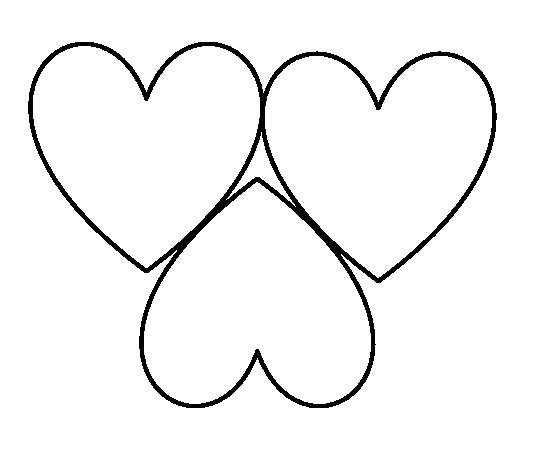
\includegraphics[width=.3\textwidth]{hearts} \quad 
	%\caption{Not valid because of gaps}
	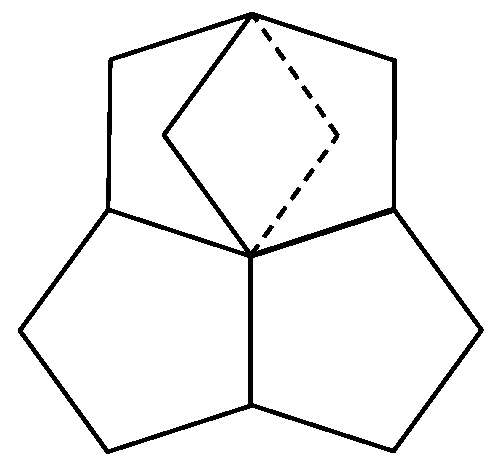
\includegraphics[width=.3\textwidth]{pentagons} \quad
	%\caption{Not valid because of overlap}
	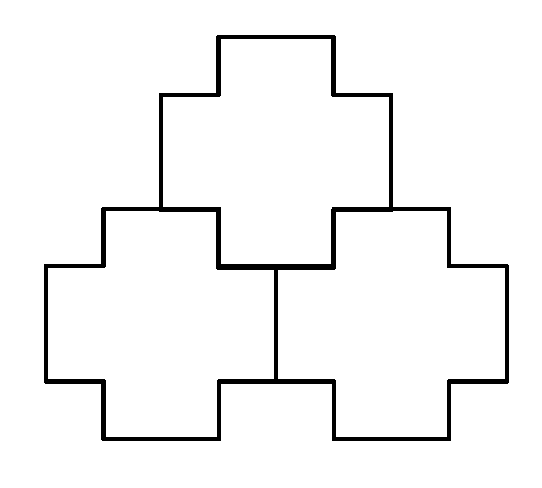
\includegraphics[width=.3\textwidth]{crosses}
	%\caption{Valid}
\end{center}

\end{question}
\mynewpage

\begin{question}
 Now we are going to use these shapes to try to create a tiling. Work
 with your groups to fill out the following table.  If you cannot
 create a tessellation with a given polygon, give the range for the
 ``number around a vertex.''

The last column is also one of the columns in the \emph{Louie Llama and the Triangle} assignment.
\begin{center}
  \renewcommand{\arraystretch}{3}
\begin{tabular}{|c||c|c|c|c|}\hline
Shape & \begin{minipage}{1in} Number of Sides \end{minipage}& \begin{minipage}{1.5in}Number around vertex\end{minipage} & Tile? & \begin{minipage}{1.5in}Interior Angle Measure\end{minipage} \\ \hline\hline
Triangle & 3 &  &  & \\ \hline
Square & 4 &  &  & \\ \hline
Pentagon & 5  &  &  & \\ \hline
Hexagon & 6 &  &  & \\ \hline
Heptagon & 7 &  &  & \\ \hline
Octagon & 8 &  &  & \\ \hline\hline
\begin{minipage}{1in}
  \begin{center}
    $n$-gon\\ $n> 8$
  \end{center}
  \end{minipage} & n &  &  & \\ \hline
\end{tabular}
\end{center}
\begin{freeResponse}
  Here is my table:
  \begin{center}
  \renewcommand{\arraystretch}{3}
\begin{tabular}{|c||c|c|c|c|}\hline
Shape & Number of Sides & Number around vertex & Tile? & Interior Angle Measure \\ \hline\hline
Triangle & $3$ & $6$ & Yes  & $60$\\ \hline
Square & $4$ & $4$  & Yes  & $90$ \\ \hline
Pentagon & $5$ & $3$--$4$ & No & $108$ \\ \hline
Hexagon & $6$ & $3$ & Yes & $120$\\ \hline
Heptagon & $7$ & $2$--$3$ &  No& $128.57$\\ \hline
Octagon & $8$ & $2$--$3$ & No & $135$\\ \hline\hline
\begin{minipage}{1in}
  \begin{center}
    $n$-gon\\ $n> 8$
  \end{center}
  \end{minipage} & $n$ & $2$--$3$ & No  & $180-\frac{360}{n}$\\ \hline
\end{tabular}
\end{center}
\end{freeResponse}
\end{question}
\mynewpage

\begin{question}
 Are these the only possible tessellations with regular polygons? If not, explain which ones are missing.
 
 Once you have a complete list, explain how you know that there are no other options.
\end{question}

\end{document}
